\documentclass[a4paper,10pt]{scrartcl}
\usepackage[utf8]{inputenc}
\usepackage{hyperref}
\renewcommand{\rmdefault}{ptm}
\usepackage{bera}% optional: just to have a nice mono-spaced font
\usepackage{listings}
\usepackage{xcolor}
\usepackage{csquotes}
\usepackage{booktabs}
\usepackage{amsfonts}
\usepackage{graphicx}
\colorlet{punct}{red!60!black}
\definecolor{background}{HTML}{EEEEEE}
\definecolor{delim}{RGB}{20,105,176}
\colorlet{numb}{magenta!60!black}

\lstdefinelanguage{json}{
    basicstyle=\normalfont\ttfamily,
    numbers=left,
    numberstyle=\scriptsize,
    stepnumber=1,
    numbersep=8pt,
    showstringspaces=false,
    breaklines=true,
    frame=lines,
    backgroundcolor=\color{background},
    literate=
     *{0}{{{\color{numb}0}}}{1}
      {1}{{{\color{numb}1}}}{1}
      {2}{{{\color{numb}2}}}{1}
      {3}{{{\color{numb}3}}}{1}
      {4}{{{\color{numb}4}}}{1}
      {5}{{{\color{numb}5}}}{1}
      {6}{{{\color{numb}6}}}{1}
      {7}{{{\color{numb}7}}}{1}
      {8}{{{\color{numb}8}}}{1}
      {9}{{{\color{numb}9}}}{1}
      {:}{{{\color{punct}{:}}}}{1}
      {,}{{{\color{punct}{,}}}}{1}
      {\{}{{{\color{delim}{\{}}}}{1}
      {\}}{{{\color{delim}{\}}}}}{1}
      {[}{{{\color{delim}{[}}}}{1}
      {]}{{{\color{delim}{]}}}}{1},
}


\newcommand{\lamine}[1]{\textcolor{blue}{#1}}
%opening
\title{DAFNA -- RestFul API for Truth Discovery Algorithms}
\subtitle{API DOCUMENTATION}
\author{\hspace*{-0.5cm}M. Lamine Ba, Hossam. H. Hammady, Laure Berti-Equille\\ \\ \sf{Qatar Computing Research institute}\\ \sf{Hamad Bin Khalifa University}\\ 
\includegraphics[scale=0.3]{qf}}

\date{\begin{tabular}{ll}Creation date:&November 5, 2015\\Revision date:&\today\end{tabular}}

\begin{document}

\maketitle
\newpage
% tableofcontents
\tableofcontents
\newpage

% Introduction
\section{Introduction}
Data Forensics with Analytics, or for short DAFNA, is a project initiated by the Data Analytics Group in Qatar Computing Research Institute, 
Hamad Bin Khalifa University.
One of its various facets aims at providing efficient algorithms and tools for verifying the veracity of information provided by multiple conflicting
sources. The DAFNA API for truth discovery is a RestFul API that enables end user applications to access and use twelve existing truth discovery algorithms
for fact checking and truth discovery when they have to integrate heterogeneous information coming from untrustworthy sources.  This documentation details
the use of the API for third-party applications.

If you use this API or related achievements such as the online tool AllegatorTrack, please do not forget to aknowledge the authors by citing \textquote{Dalia Attia Waguih, Naman Goel, Hossam M. Hammady,
Laure Berti-Equille. AllegatorTrack: Combining and Reporting Results of Truth Discovery from Multi-source Data. The 31th International Conference on Data Engineering (ICDE), 
Seoul, Korea, 2015}. 




% Authentication
\section{Authentication}
Third party developers wanting to test DAFNA API for truth discovery, or integrate it in their own applications,
need to first get the necessary access credentials. To obtain credentials, every 3rd party developer must
follows the process below.
\begin{itemize}
 \item Go to \href{http://dafna.qcri.org/users/sign_in}{AllegatorTrack}
 \item Register using a valid email id and email confirmation
 \item Contact DAFNA developers for token access.
\end{itemize}
 Upon token access request done, the user will receive from DAFNA developpers the following access credentials.
\begin{itemize}
 \item \textbf{Authentication Token}: API user's access key
 \item \textbf{Encrypted Password}: user's secret key
\end{itemize}

% Dataset Format
\section{Dataset Format}\label{dataset_format}
All the datasets used as input through the API must be CVS files having one of the two following header lines (the order between column names is important
and must be respected).
\begin{enumerate}
 \item[1.] \textbf{ObjectID, PropertyID, PropertyValue, SourceID, TimeStamp}
\end{enumerate}

For instance given in a flight dataset, we obtain using (1):\\ 

 \scriptsize
{
 \begin{tabular}{l}
\textquote{\textbf{ObjectID}},~\textquote{\textbf{PropertyID}},~\textquote{\textbf{PropertyValue}},~\textquote{\textbf{SourceID}},~\textquote{\textbf{TimeStamp}}\\
\textquote{AA-1623-EWR-MIA2011-12-18},~\textquote{ActualDepartureTime},~\textquote{12/18/11 2:58 PM (-05:00)},~\textquote{myrateplan},~\textquote{2011-12-18}\\
\textquote{AA-1623-EWR-MIA2011-12-18},~\textquote{ActualArrivalTime},~\textquote{12/18/11 5:14 PM (-05:00)},~\textquote{myrateplan},~\textquote{2011-12-18}\\
\textquote{AA-1623-EWR-MIA2011-12-18},~\textquote{ActualDepartureTime},~\textquote{12/18/11 2:58 PM (-05:00)},~\textquote{helloflight},~\textquote{2011-12-18}\\
\textquote{AA-1623-EWR-MIA2011-12-18},~\textquote{ActualArrivalTime},~\textquote{12/18/11 5:14 PM (-05:00)},~\textquote{helloflight},~\textquote{2011-12-18}
\end{tabular}
}

\normalsize
\begin{enumerate}
 \item[2.] \textbf{ObjectID, PropertyID, PropertyValues, SourceID, TimeStamp}
\end{enumerate}

Given a book dataset with a property having multiple values, we obtain using (2):\\

 \scriptsize
{
 \begin{tabular}{l}
\textquote{\textbf{ObjectID}},~\textquote{\textbf{PropertyID}},~\textquote{\textbf{PropertyValues}},~\textquote{\textbf{SourceID}},~\textquote{\textbf{TimeStamp}}\\
\textquote{0023606924},~\textquote{AuthorName},~\textquote{schaefer.~marcus, johnsonbaugh.~richard},~\textquote{a1books},~\textquote{null}\\
\textquote{0023606924},~\textquote{AuthorName},~\textquote{schaefer.~marcus, johnsonbaugh.~richard},~\textquote{alinonline},~\textquote{null}\\
\textquote{0023606924},~\textquote{AuthorName},~\textquote{schaefer,~marcus, johnsonbaugh.~richard},~\textquote{california textbooks},~\textquote{null}\\
\textquote{0023606924},~\textquote{AuthorName},~\textquote{johnsonbaugh.~richard},~\textquote{deepak sachdeva},~\textquote{null}\\ \\
\end{tabular}
}


\normalsize
If the dataset adopts the second type of header line, the system will automatically split the contents of this 
column on the comma when running multi-valued algorithms.

As for the ground truth datasets they must be a CSV file with a header line having the following column
names in any order: \textbf{ObjectID, PropertyID, PropertyValue}. Note that the values in \textbf{ObjectID} should match those in the 
corresponding dataset file so that objects are correctly matched (case sensitive). Again, you can replace
\textbf{PropertyValue} by \textbf{PropertyValues} and the system will automatically split the contents of this column on the 
comma when running multi-valued algorithms. Below is an example of a ground truth dataset formatting.\\

\scriptsize
{
\begin{tabular}{l}
\textquote{\textbf{ObjectID}},~\textquote{\textbf{PropertyID}},~\textquote{\textbf{PropertyValue}}\\
\textquote{AA-1221-MCO-ORD2011-12-01},~\textquote{ExpectedDepartureTime},~\textquote{12/01/2011 08:00 PM}\\
\textquote{AA-1221-MCO-ORD2011-12-01},~\textquote{ActualDepartureTime},~\textquote{12/01/2011 08:23 PM}\\
\textquote{AA-1221-MCO-ORD2011-12-01},~\textquote{DepartureGate},~\textquote{17}\\
\textquote{AA-1221-MCO-ORD2011-12-01},~\textquote{ExpectedArrivalTime},\textquote{12/01/2011 09:45 PM}\\
\end{tabular}
}

\normalsize


% Request format
\section{Request Format}
% Scheme
\subsection{Scheme}
Requests to the API endpoints are done using plain HTTP. HTTPS is planned to be supported 
in the future development of the API for ensuring a more secure transmission of the Access 
Token.
% Methods
\subsection{Methods}
The current version of DAFNA API supports three HTTP Requests, i.e., \textbf{GET}, \textbf{POST}, and \textbf{DELETE}, 
with respect to the operations, for instance creation, listing, or removal of datasets, the 3rd party applications would
like to perform on the behalf on the client.
% Base Url
\subsection{Base URL}
The API is accessible through the following base URL.
\begin{itemize}
 \item \href{http://dafna.qrci.org/}{http://dafna.qrci.org/}
\end{itemize}
Every endpoint of the API must be appended to this given base URL.
For instance, to list the set of available datasets, client must use 
the following URL.
\begin{description}
\item GET \href{http://dafna.qcri.org/datasets/}{http://dafna.qcri.org/datasets/} 
\end{description}
% Request content type
\subsection{Request Content Type}
Either (1) \textquote{application/x-www-form-urlencoded} or (2) \textquote{application/json} can be used as the request content type (HTTP request \textquote{Content-Type}
header value). If (1) is used, all parameters should be encoded in the URL as a query string with proper escapes and separated by \&. If (2) is used, the request body should 
be a well-formed JSON object. 

\begin{enumerate}
 \item \textbf{url-encoded form}
\begin{description}
 \item POST \href{http://localhost:4000/runsets?checked\_algo=array\_of\_parameters}{http://dafna.qcri.org/runsets?checked\_algo=array\_of\_parameters}
\end{description}
 \item \textbf{json encoding}
\begin{description}
 \item POST \href{http://localhost:4000/runsets}{http://dafna.qcri.org/runsets}~
 \{checked\_algo: array\_of\_parameters, general\_config: array\_numerical\_values\}
\end{description}
\end{enumerate}

Note that when using some command line tools to issue your requests, the way the body content is passed could be slighted different.
For example, when a particular user issues requests through command lines via
\href{http://curl.haxx.se/}{\textquote{Curl}}, (1) and (2) argument passing techniques are respectively implemented as follows.
\begin{description}
 \item curl -X DELETE http://dafna.qcri.org/runsets/1/ -d \textquote{user\_token=some\_string\_here}\\
 \item and \\
 \item curl -X POST http://dafna.qcri.org/runsets -H ``Content-type: application/json" -d `\{\textquote{user\_token}: \textquote{some\_string\_here}, \textquote{datasets}: \{\textquote{dataset\_id}:\textquote{1}, \textquote{gt\_id}:\textquote{1}\}, \textquote{checked\_algo}: \{\textquote{Accu}: [\textquote{0.2}, \textquote{0}, \textquote{100}, \textquote{0.5}, \textquote{false}, \textquote{true}, \textquote{true}, \textquote{false}] \}, \textquote{general\_config}:[\textquote{0.001}, \textquote{0.8}, \textquote{1}, \textquote{0.4}]\}' 
\end{description}
% Response format
\section{Response Format}
% http status code
\subsection{HTTP Status Codes}
\begin{itemize}
 \item \textbf{200:} Successful Requests (otherwise, an internal error will occur)
 \item \textbf{401:} Unauthorized Access, e.g., missing, invalid, or expired token
 \item \textbf{403:} Forbidden Access to the resource requested by the client
 \item \textbf{404:} Not Found Resource requested by the user
 \item \textbf{422:} Invalid Action on the accessed resource
 
\end{itemize}

% Response body format
\subsection{Response Body Format}
Responses to user queries are returned in JSON format. For now, JSON is the only supported format by the API for query output.
Further development might consider other formats such as XML.

% endpoints 
\section{Endpoints}
The current version of the API provides 8 endpoints, 4 among them are accessed via GET, 2 via POST, and 2 via DELETE:
% post endpoints
\subsection{POST Endpoints}
\begin{enumerate}
 \item \textbf{/datasets}
\begin{description}
 \item Requests the creation of a Dataset
\end{description}
\textbf{Parameters}
\begin{itemize}
\item \textbf{user\_token}: secret token provided to the client for authentication 
\item \textbf{s3\_key}: a file's s3 key if the file is uploaded at Amazon's s3 official. Right access to this bucket 
is needed.
\item \textbf{other\_url}: URL (other than the s3 key) if the dataset file is located somewhere else, e.g. in a local computer.
\item \textbf{kind}: either \textquote{claims} or \textquote{ground} corresponding to the different types of handled datasets
\item \textbf{original\_filename}: name of the uploaded file. It corresponds to any name that you want to give for identification
in future
\end{itemize}
\textbf{Response}
\begin{description}
 \item No data. 
 \item \textbf{200} status code when the request succeeds	
\end{description}
\textbf{Notes}
\begin{enumerate}
 \item One of \textbf{s3\_key} or \textbf{other\_url} parameters are mandatory for parsing dataset. 
 \item All uploaded files should be encoded in \textbf{UTF-8}.
 \item Be sure that your dataset fulfills the required format as described in Section~\ref{dataset_format}.
\end{enumerate}
%\textbf{Example}
%\begin{description}
% \item Curl -X POST \textquote{http://dafna.qcri.org/datasets}
% -H \textquote{Content-Type: application/x-www-form-urlencoded; charset=UTF-8}
% -d \textquote{user\_token=oMeqs5h\_zfsTXnTks4PS}
% -d \textquote{s3\_key=import\%2F1fa3e133-365e-427f-b490-8753c42f1478\%2Fclaims4.csv}
% -d \textquote{original\_filename=claims4.csv} -d \textquote
%\end{description}
  
%\lamine{POST not yet finish !}
%
 \item \textbf{/runsets}
 \begin{description}
 \item Creating a Runset, i.e., a truth discovery job over a given dataset
\end{description}
\textbf{Parameters}
\begin{itemize}
 \item \textbf{user\_token}: secret token provided to the client for authentication 
 \item \textbf{datasets}: list of dataset identiers referring to the datasets on which the runset should applied. An example
 input is \textbf{datasets}:\{\textquote{203}:\textquote{1}, \textquote{204}:\textquote{1}\} denoting the choice of the dataset
 numbered 203 along with the corresponding ground truth dataset with the number 204. 
 \item  \textbf{checked\_algo}: set of algorithm name(s), each followed by an array of numerical values 
 for its different input parameters, e.g., \textquote{checked\_algo}: \{\textquote{Accu}: [\textquote{0.2}, \textquote{0}, \textquote{100}, \textquote{0.5}, \textquote{false}, \textquote{true}, \textquote{true}, \textquote{false}] , \textquote{Cosine}: [\textquote{1}, \textquote{0.2}] \}
specifies two algorithms \textbf{Accu} and \textbf{Cosine}
 \item \textbf{general\_config}: an array of numerical values, e.g., [\textquote{0.001}, \textquote{0.8}, \textquote{1}, \textquote{0.4}]
\end{itemize}
\textbf{Response}
\begin{description}
\item No data. 
 \item \textbf{200} status code when request succeed.	
\end{description}
\textbf{Notes}
\begin{enumerate}
 \item \textbf{checked\_algo} allows to specify the set of truth discovery algorithms along with the values of their input arguments to be used for the truth discovery process. At least one algorithm must be provided, and when several algorithms
 are specified their results are combined by the system for a better accuracy. We detail in Section~\ref{algorithms} the set of supported truth discovery algorithms together with their input arguments.
 %To see the details of all truth discovery algorithms supported by the API, please visit the following page: \href{http://daqcri.github.io/dafna/\#/dafna/exp\_sections/home.html}{http://daqcri.github.io/dafna/\#/dafna/exp\_sections/home.html}.
\item \textbf{general\_config} allows to specify the values of the general parameters of a runset, i.e., the convergence test thresold and the initial sources' trusworthiness scores.
 \end{enumerate}
\end{enumerate}

% get endpoints
\subsection{GET Endpoints}
\begin{enumerate}
 \item \textbf{/datasets}
\begin{description}
 \item Listing Datasets 
\end{description}
\textbf{Parameters}
\begin{itemize}
\item \textbf{user\_token}: secret token provided to the client for authentication
\item \textbf{kind}: either \textquote{claims} or \textquote{ground} which correspond to the different types of available datasets
\item \textbf{start}: an integer number specifying the index from which the listing of available datasets must start 
\item \textbf{length}: an integer specifying the maximum number of datasets to be listed
\end{itemize}
\textbf{Response}
\begin{description}
 \item \{DS$_1$, DS$_2$, $\ldots$, DS$_n$\} where every DS$_n$ is formatted as follows.\\ \\
 \{
  draw: $<$draw$>$,
  recordsTotal: $<$Number of Records$>$,
  recordsFiltered: $<$Number of filtered Records$>$,
  data: $<$data$>$,
  s3\_direct\_post: $<$date\_time$>$,
  fields: $<$date\_time$>$,
  key: $<$date\_time$>$,
  policy: $<$policy$>$,
  signature: $<$signatur$>$,
  success\_action\_status: $<$status$>$
\}\\ \\
\hspace*{-1cm} where $<$data$>$ contains all the information about to the available datasets.
\end{description}
\textbf{Notes}
\begin{enumerate}
 \item \textbf{start} and \textbf{length} parameters are optional. 
 \item When the parameter \textbf{kind} is not provided, the user will get an empty 
 set of datasets. 
 \item When the arguments \textbf{start} and \textbf{length} 
 are not specified, all the available datasets of the specified kind are returned.
\end{enumerate}

%
\item \textbf{/runsets}
\begin{description}
 \item Listing Runsets
\end{description}
\textbf{Parameters}
\begin{itemize}
 \item \textbf{user\_token}: secret token provided to the client for authentication
\end{itemize}
\textbf{Response:}
\begin{description}
 \item \{RS$_1$, RS$_2$, $\cdots$, RS$_n$\} where the format of RS$_n$ is:\\
\{
  id: $<$runset id$>$,
  created\_at: $<$Time of creation$>$,
  runs:[ 
\{
  id: $<$runset id$>$,
  algo: $<$Time of creation$>$,
  crated\_at: $<>$,
  status: $<$whether finished$>$,
  duration: $<$Duration of run$>$,
\}
,\{\},\{\}...]
\}	
\end{description}
%
\item \textbf{/runsets/<id>/results}
\begin{description}
 \item Listing Results of runsets having id=<id>
\end{description}
\textbf{Parameters}
\begin{itemize}
 \item \textbf{user\_token}: secret token provided to the client for authentication
 \item \textbf{id}: an existing identier of the runset whose results should be listed
\end{itemize}
\textbf{Response}
\begin{description}
 \item
 \{
  draw: $<$draw$>$,
  recordsTotal: $<$Total Number of Records$>$,
  recordsFiltered: $<$Filtered Records$>$,
  data: 

\}
\end{description}
%
\item \textbf{/runs}
\begin{description}
\item Listing Runs
\end{description}
\textbf{Parameters}
\begin{itemize}
 \item \textbf{user\_token}: secret token provided to the client for authentication
\end{itemize}
\textbf{Response}
\begin{description}
\item 
\{
  draw: $<$draw$>$,
  recordsTotal: $<$Total Number of Records$>$,
  recordsFiltered: $<$Filtered Records$>$,
  data:[ \{
  id: $<$run id$>$,
  algorithm: $<$Name of the algorithm$>$,
  created\_at: $<$Time of creation$>$,
  runset\_id: $<$Runset ID$>$,
  display: $<$Algorithm name and parameters in paranthesis (in order)$>$,
  status: $<$whether finished$>$,
  duration: $<$Duration of run$>$,
\}
,\{\},\{\}...]
\}	
\end{description}
\end{enumerate}

% post endpoints
\subsection{DELETE Endpoints}
\begin{enumerate}
\item \textbf{/datasets/<id>}
\begin{description}
 \item Deleting a Dataset having id=<id>
\end{description}
\textbf{Parameters}
\begin{itemize}
 \item \textbf{user\_token}: secret token provided to the client for authentication
 \item \textbf{id}: an existing identier of the dataset to be deleted 
\end{itemize}
\textbf{Response}
\begin{description}
 \item No data.
\item  \textbf{200} status code when the request succeeds.
\end{description}
%
\item \textbf{/runsets/<id>}
\begin{description}
\item Deleting a Runset having id=<id>
\end{description}
\textbf{Parameters}
\begin{itemize}
  \item \textbf{user\_token}: secret token provided to the client for authentication
 \item \textbf{id}: an existing identier of the runset to be deleted 
\end{itemize}
\textbf{Response}
\begin{description}
\item  No data.
\item \textbf{200} status code when the request succeeds.	
\end{description}
\end{enumerate}

% Algorithm names
\section{Supported Algorithms}\label{algorithms}
The main interest of using the API is to create a truth discovery job which is possible with an instantiation 
of a runset. Such a instantiation requires to specify one or more truth discovery algorithms to use through the
argument \textbf{checked\_algo}. In the following, we detail the twelve truth discovery algorithms 
and their specific input parameters supported by DAFNA API. 

\subsection{Cosine}
\begin{description}
\item \textbf{Description}: Cosine is a heuristic approach for estimating a value confidence and source trustworthiness, based on the cosine similarity measure proposed by A. Galland, S. Abiteboul, A. Marian, and P. Senellart. Corroborating Information from Disagreeing Views. In WSDM, pp. 131–140, 2010.
\item \textbf{Parameters}
\begin{itemize}
\item \textbf{Initial Value Confidence}: Initialization of value confidence for all properties values.
\item[]\textbf{dataType: }double, \textbf{min-value: }0, \textbf{max-value: }1.0, \textbf{default-value: }1\item \textbf{Prediction constant}: Constant that gives more weight to predictable views (eg, sources with consistently often correct claims or consistently often wrong claims).
\item[]\textbf{dataType: }double, \textbf{min-value: }0, \textbf{max-value: }1, \textbf{default-value: }0.2\end{itemize}
\end{description}
\subsection{2-Estimates}
\begin{description}
\item \textbf{Description}: 2-Estimates is a probabilistic model built over the heuristic model, Cosine and proposed by A. Galland, S. Abiteboul, A. Marian, and P. Senellart. Corroborating Information from Disagreeing Views. In WSDM, pp. 131–140, 2010.
\item \textbf{Parameters}
\begin{itemize}
\item \textbf{Normalization Factor}: The weight used for normalizing sources' trustworthiness and values' confidence.
\item[]\textbf{dataType: }double, \textbf{min-value: }0, \textbf{max-value: }1, \textbf{default-value: }0.5\end{itemize}
\end{description}
\subsection{3-Estimates}
\begin{description}
\item \textbf{Description}: 3-Estimates extends 2-Estimates proposed by A. Galland, S. Abiteboul, A. Marian, and P. Senellart. Corroborating Information from Disagreeing Views. In WSDM, pp. 131–140, 2010.
\item \textbf{Parameters}
\begin{itemize}
\item \textbf{Initial Error Factor}: Initialization of value's error factor for all properties values.
\item[]\textbf{dataType: }double, \textbf{min-value: }0, \textbf{max-value: }1.0, \textbf{default-value: }0.4\item \textbf{Normalization Factor}: The constant used for normalizing source truthworthiness and value confidence.
\item[]\textbf{dataType: }double, \textbf{min-value: }0, \textbf{max-value: }1, \textbf{default-value: }0.5\end{itemize}
\end{description}
\subsection{Depen}
\begin{description}
\item \textbf{Description}: First Bayesian truth discovery model that takes into cosideration the copying relationship between sources, proposed by X. L. Dong, L. Berti-Equille, and D. Srivastava. Integrating conflicting data: The role of source dependence. PVLDB, 2(1):550–561, 2009.
\item \textbf{Parameters}
\begin{itemize}
\item \textbf{Dependence priori probability}: The a priori probability that two data sources are dependent.
\item[]\textbf{dataType: }double, \textbf{min-value: }0, \textbf{max-value: }0.5, \textbf{default-value: }0.2\item \textbf{Copied value probability}: The probability that a value provided by a copier is copied.
\item[]\textbf{dataType: }double, \textbf{min-value: }0, \textbf{max-value: }1, \textbf{default-value: }0\item \textbf{Number of false values}: The number of false values in the underlying domain for each object.
\item[]\textbf{dataType: }int, \textbf{min-value: }1, \textbf{max-value: }1, \textbf{default-value: }100\item \textbf{Similarity Constant}: The similarity betwen values is weighted for the value confidence computation.
\item[]\textbf{dataType: }double, \textbf{min-value: }0, \textbf{max-value: }1, \textbf{default-value: }0.5, \textbf{hidden: }True
\item \textbf{considerSimilarity}: False for Depen: the model does not take into account value similarity.
\item[]\textbf{dataType: }boolean, \textbf{min-value: }0, \textbf{max-value: }1, \textbf{default-value: }False, \textbf{hidden: }True
\item \textbf{considerSourcesAccuracy}: False for Depen: the model does not take into account the accuracy of the sources.
\item[]\textbf{dataType: }boolean, \textbf{min-value: }0, \textbf{max-value: }1, \textbf{default-value: }False, \textbf{hidden: }True
\item \textbf{considerDependence}: True for Depen: the model takes into account the dependence between sources.
\item[]\textbf{dataType: }boolean, \textbf{min-value: }0, \textbf{max-value: }1, \textbf{default-value: }True, \textbf{hidden: }True
\item \textbf{orderSrcByDependence}: If true, Depen model is based on source dependence ordering, otherwise on lexicographic ordering.
\item[]\textbf{dataType: }boolean, \textbf{min-value: }0, \textbf{max-value: }1, \textbf{default-value: }False, \textbf{hidden: }True
\end{itemize}
\end{description}
\subsection{Accu}
\begin{description}
\item \textbf{Description}: Accu extends Depen model and considers the source accuracy in addition to the source dependence, proposed by X. L. Dong, L. Berti-Equille, and D. Srivastava. Integrating conflicting data: The role of source dependence. PVLDB, 2(1):550–561, 2009.
\item \textbf{Parameters}
\begin{itemize}
\item \textbf{Dependence a priori probability}: The a priori probability that two data sources are dependent.
\item[]\textbf{dataType: }double, \textbf{min-value: }0, \textbf{max-value: }0.5, \textbf{default-value: }0.2\item \textbf{Copied value probability}: The probability that a value provided by a copier is copied.
\item[]\textbf{dataType: }double, \textbf{min-value: }0, \textbf{max-value: }1, \textbf{default-value: }0\item \textbf{Number of false values}: The number of false values in the underlying domain for each object.
\item[]\textbf{dataType: }int, \textbf{min-value: }1, \textbf{max-value: }1, \textbf{default-value: }100\item \textbf{Similarity Constant}: The similarity betwen values is weighted for the value confidence computation.
\item[]\textbf{dataType: }double, \textbf{min-value: }0, \textbf{max-value: }1, \textbf{default-value: }0.5, \textbf{hidden: }True
\item \textbf{considerSimilarity}: False for Accu: the model does not take into account value similarity.
\item[]\textbf{dataType: }boolean, \textbf{min-value: }0, \textbf{max-value: }1, \textbf{default-value: }False, \textbf{hidden: }True
\item \textbf{considerSourcesAccuracy}: True for Accu: the model takes into account the accuracy of the sources.
\item[]\textbf{dataType: }boolean, \textbf{min-value: }0, \textbf{max-value: }1, \textbf{default-value: }True, \textbf{hidden: }True
\item \textbf{considerDependency}: True for Accu: the model takes into account the dependence between sources.
\item[]\textbf{dataType: }boolean, \textbf{min-value: }0, \textbf{max-value: }1, \textbf{default-value: }True, \textbf{hidden: }True
\item \textbf{orderSrcByDependence}: If true, Accu model is based on source dependence ordering, otherwise on lexicographic ordering.
\item[]\textbf{dataType: }boolean, \textbf{min-value: }0, \textbf{max-value: }1, \textbf{default-value: }False, \textbf{hidden: }True
\end{itemize}
\end{description}
\subsection{AccuSim}
\begin{description}
\item \textbf{Description}: Accusim extends Accu model and considers the value similarity, proposed by X. L. Dong, L. Berti-Equille, and D. Srivastava. Integrating conflicting data: The role of source dependence. PVLDB, 2(1):550–561, 2009.
\item \textbf{Parameters}
\begin{itemize}
\item \textbf{Dependence a priori probability}: The a priori probability that two data sources are dependent.
\item[]\textbf{dataType: }double, \textbf{min-value: }0, \textbf{max-value: }0.5, \textbf{default-value: }0.2\item \textbf{Copied value probability}: The probability that a value provided by a copier is copied.
\item[]\textbf{dataType: }double, \textbf{min-value: }0, \textbf{max-value: }1, \textbf{default-value: }0\item \textbf{Number of false values}: The number of false values in the underlying domain for each object.
\item[]\textbf{dataType: }int, \textbf{min-value: }1, \textbf{max-value: }1, \textbf{default-value: }100\item \textbf{Similarity Constant}: The similarity betwen values is weighted for the value confidence computation.
\item[]\textbf{dataType: }double, \textbf{min-value: }0, \textbf{max-value: }1, \textbf{default-value: }0.5\item \textbf{considerSimilarity}: True for AccuSim: the model takes into account value similarity.
\item[]\textbf{dataType: }boolean, \textbf{min-value: }0, \textbf{max-value: }1, \textbf{default-value: }True, \textbf{hidden: }True
\item \textbf{considerSourcesAccuracy}: True for AccuSim: the model takes into account the accuracy of the sources.
\item[]\textbf{dataType: }boolean, \textbf{min-value: }0, \textbf{max-value: }1, \textbf{default-value: }True, \textbf{hidden: }True
\item \textbf{considerDependency}: True for Accusim: the model takes into account the dependence between sources.
\item[]\textbf{dataType: }boolean, \textbf{min-value: }0, \textbf{max-value: }1, \textbf{default-value: }True, \textbf{hidden: }True
\item \textbf{orderSrcByDependence}: If true, AccuSim model is based on source dependence ordering, otherwise on lexicographic ordering.
\item[]\textbf{dataType: }boolean, \textbf{min-value: }0, \textbf{max-value: }1, \textbf{default-value: }False, \textbf{hidden: }True
\end{itemize}
\end{description}
\subsection{AccuNoDep}
\begin{description}
\item \textbf{Description}: AccuNoDep extends Accu model while assuming all sources are independent, proposed by X. L. Dong, L. Berti-Equille, and D. Srivastava. Integrating conflicting data: The role of source dependence. PVLDB, 2(1):550–561, 2009.
\item \textbf{Parameters}
\begin{itemize}
\item \textbf{Dependence a priori probability}: The a priori probability that two data sources are dependent.
\item[]\textbf{dataType: }double, \textbf{min-value: }0, \textbf{max-value: }0.5, \textbf{default-value: }0.2\item \textbf{Copied value probability}: The probability that a value provided by a copier is copied.
\item[]\textbf{dataType: }double, \textbf{min-value: }0, \textbf{max-value: }1, \textbf{default-value: }0\item \textbf{Number of false values}: The number of false values in the underlying domain for each object.
\item[]\textbf{dataType: }int, \textbf{min-value: }1, \textbf{max-value: }1, \textbf{default-value: }100\item \textbf{Similarity Constant}: The similarity betwen values is weighted for the value confidence computation.
\item[]\textbf{dataType: }double, \textbf{min-value: }0, \textbf{max-value: }1, \textbf{default-value: }0.5, \textbf{hidden: }True
\item \textbf{considerSimilarity}: False for AccuNoDep: the model does not take into account value similarity.
\item[]\textbf{dataType: }boolean, \textbf{min-value: }0, \textbf{max-value: }1, \textbf{default-value: }False, \textbf{hidden: }True
\item \textbf{considerSourcesAccuracy}: True for AccuNoDep: the model takes into account the accuracy of the sources.
\item[]\textbf{dataType: }boolean, \textbf{min-value: }0, \textbf{max-value: }1, \textbf{default-value: }True, \textbf{hidden: }True
\item \textbf{considerDependency}: False for AccuNoDep: the model considers that all sources are independent.
\item[]\textbf{dataType: }boolean, \textbf{min-value: }0, \textbf{max-value: }1, \textbf{default-value: }False, \textbf{hidden: }True
\item \textbf{orderSrcByDependence}: If true, AccuNoDep model is based on source dependence ordering, otherwise on lexicographic ordering.
\item[]\textbf{dataType: }boolean, \textbf{min-value: }0, \textbf{max-value: }1, \textbf{default-value: }False, \textbf{hidden: }True
\end{itemize}
\end{description}
\subsection{TruthFinder}
\begin{description}
\item \textbf{Description}: TruthFinder, proposed by X. Yin, J. Han, and P. S. Yu. Truth Discovery with Multiple Conflicting Information Providers on the Web. TKDE, 20(6):796–808, 2008, is a Bayesian model that iteratively computes and updates the trustworthiness of a source as a function of the belief in its claims, and then the belief score of each claim as a function of the trustworthiness of the sources asserting it.
\item \textbf{Parameters}
\begin{itemize}
\item \textbf{Similarity Constant}: The similarity betwen values is weighted for the value confidence computation.
\item[]\textbf{dataType: }double, \textbf{min-value: }0, \textbf{max-value: }1, \textbf{default-value: }0.5\item \textbf{Dampening Factor}: The damping factor compensates the effect when sources with similar values are actually dependent.
\item[]\textbf{dataType: }double, \textbf{min-value: }0, \textbf{max-value: }1, \textbf{default-value: }0.1\end{itemize}
\end{description}
\subsection{SimpleLCA}
\begin{description}
\item \textbf{Description}: SimpleLCA (Latent Credibility Analysis) is a probabilistic model proposed by J. Pasternack and D. Roth. Latent Credibility Analysis. In WWW, pp. 1009–1020, 2013. Each source has a probability of being honest, and all sources are considered independent.
\item \textbf{Parameters}
\begin{itemize}
\item \textbf{Prior truth probability}: Prior probability of a claim being the true claim.
\item[]\textbf{dataType: }double, \textbf{min-value: }0, \textbf{max-value: }1, \textbf{default-value: }0.5\end{itemize}
\end{description}
\subsection{GuessLCA}
\begin{description}
\item \textbf{Description}: GuessLCA extends SimpleLCA by adding a probability of a source guessing the true value while being honest.
\item \textbf{Parameters}
\begin{itemize}
\item \textbf{Prior truth probability}: Prior probability of a claim being the true claim.
\item[]\textbf{dataType: }double, \textbf{min-value: }0, \textbf{max-value: }1, \textbf{default-value: }0.5\end{itemize}
\end{description}
\subsection{MLE}
\begin{description}
\item \textbf{Description}: MLE (Maximum Likelihood Estimation) proposed by D. Wang, L. M. Kaplan, H. K. Le, and T. F. Abdelzaher. On Truth Discovery in Social Sensing: a Maximum Likelihood Estimation Approach. In IPSN, pp. 233–244, 2012, is based on the Expectation Maximization (EM) algorithm to quantify the reliability of sources and the correctness of their observations. It only deals with boolean positive attributes observations.
\item \textbf{Parameters}
\begin{itemize}
\item \textbf{Prior truth probability}: Overall prior probability of the claims being the true claims.
\item[]\textbf{dataType: }double, \textbf{min-value: }0, \textbf{max-value: }1, \textbf{default-value: }0.5\item \textbf{r}: The probability that a source provides a value for all data items.
\item[]\textbf{dataType: }double, \textbf{min-value: }0, \textbf{max-value: }1, \textbf{default-value: }0.5\end{itemize}
\end{description}
\subsection{LTM}
\begin{description}
\item \textbf{Description}: LTM (Latent Truth Model) proposed by B. Zhao, B. I. P. Rubinstein, J. Gemmell, and J. Han. A Bayesian Approach to Discovering Truth from Conflicting Sources for Data Integration. PVLDB, 5(6):550–561, 2012, uses Bayesian Networks for estimating the truth. LTM iterates over a fixed number of iterations, and compute the value confidence using Collapsed Gibbs Sampling process.
\item \textbf{Parameters}
\begin{itemize}
\item \textbf{Prior truth probability}: Prior probability of how likely each claim is to be true.
\item[]\textbf{dataType: }double, \textbf{min-value: }0.0, \textbf{max-value: }1.0, \textbf{default-value: }0.5\item \textbf{Prior falsehood probability}: Prior probability of how likely each claim is to be false.
\item[]\textbf{dataType: }double, \textbf{min-value: }0.0, \textbf{max-value: }1.0, \textbf{default-value: }0.5\item \textbf{Prior true negative count}: Prior number of true negatives for the sources.
\item[]\textbf{dataType: }double, \textbf{min-value: }0.0, \textbf{max-value: }1.0, \textbf{default-value: }0.1\item \textbf{Prior false positive count}: Prior number of false positives for the sources.
\item[]\textbf{dataType: }double, \textbf{min-value: }0.0, \textbf{max-value: }1.0, \textbf{default-value: }0.9\item \textbf{Prior false negative count}: Prior number of false negatives for the sources.
\item[]\textbf{dataType: }double, \textbf{min-value: }0.0, \textbf{max-value: }1.0, \textbf{default-value: }0.1\item \textbf{Prior true positive count}: Prior number of true positives for the sources.
\item[]\textbf{dataType: }double, \textbf{min-value: }0.0, \textbf{max-value: }1.0, \textbf{default-value: }0.9\item \textbf{Number Of Iterations}: Number of Iterations.
\item[]\textbf{dataType: }int, \textbf{min-value: }1, \textbf{max-value: }10000, \textbf{default-value: }500\item \textbf{Burn-in}: Collapsed Gibbs Sampling burn-in period (ie, the number of discarded first set of iterations) must be significantly less than the number of iterations.
\item[]\textbf{dataType: }int, \textbf{min-value: }0, \textbf{max-value: }1000, \textbf{default-value: }100\item \textbf{Thinning}: Collapsed Gibbs Sampling thinning parameter (ie, the number of iterations to be skipped every time before considering the result of a selected iteration) 
must be significantly less than the number of iterations.
\item[]\textbf{dataType: }int, \textbf{min-value: }0, \textbf{max-value: }1000, \textbf{default-value: }9\end{itemize}
\end{description}
\paragraph*{$^{\dagger}$General Parameters.}
Parameters needed for all Truth Discovery Algorithms (specified via the \textbf{general\_config} parameter)
\begin{description}
\item \textbf{Parameters}
\begin{itemize}
\item \textbf{Convergence test threshold}: The difference of source truthworthiness cosine similarity between two successive iterations should be less than the user-defined threshold.
\item[]\textbf{dataType: }double, \textbf{min-value: }0, \textbf{max-value: }0.1, \textbf{default-value: }0.001, \textbf{step: }0.001\item \textbf{Initial sources truthworthiness}: Initialization of all sources truthworthiness.
\item[]\textbf{dataType: }double, \textbf{min-value: }0, \textbf{max-value: }1.0, \textbf{default-value: }0.8\item \textbf{Initial Value Confidence}: Initialization of value confidence for all properties values.
\item[]\textbf{dataType: }double, \textbf{min-value: }0, \textbf{max-value: }1.0, \textbf{hidden: }True
\item \textbf{Initial Error Factor}: Initialization of error factor for all properties values.
\item[]\textbf{dataType: }double, \textbf{min-value: }0, \textbf{max-value: }1.0, \textbf{default-value: }0.4, \textbf{hidden: }True
\end{itemize}
\end{description}
\paragraph*{$^{\dagger}$Combiner.}
The combiner of selected truth discovery algorithms. It is automatically selected if you select more than 1 algorithm and 1 ground truth dataset. It is based on Bayes combination from P. Domingos and M. Pazzani. On the optimality of the simple Bayesian classifier under zero-one loss. Machine Learning, 29:103–130, 1997.
% API Usage : use case
\section{DAFNA API Usage: Use Case}
Let us consider a typical scenario where a given user, holding an access token \textbf{\textquote{\_XYH128PL04}} to the DAFNA API, would 
like to discover the correct list of authors of a set of books. The user has first extracted the candidate authors of
these books from different Web sources and has stored them into a csv file \textbf{book.csv} in a local directory named \textbf{./datasets/}.
To discover the truth using our API, the user needs to upload (or create) the dataset, get the dataset identifier, create a runset (using \textbf{Accu} algorithm),
get the runset identifier, and finally view the result of this runset. The user can further decide to delete the copy of the dataset on the server. To this end, 
she (or he) should issues following sequence of requests.
\begin{enumerate}
 \item curl -X POST http://dafna.qcri.org/datasets -H  \textquote{Content-Type: application/x-www-form-urlencoded; charset=UTF-8} 
  -d \textquote{user\_token=\_XYH128PL04} -d \textquote{other\_url=./dataset/book.csv} -d \textquote{original\_filename=book.csv\&kind=claims} (upload the dataset of the server)
 \item curl -X GET http://dafna.qcri.org/datasets -d \textquote{user\_token=\_XYH128PL04} -d \textquote -d \textquote{start=0} 
 -d \textquote{length=54} (list the set of datasets on the server: let's assume that this returns the book dataset with the identifier \textbf{\textquote{120}})
 \item curl -X POST http://dafna.qcri.org/runsets -H ``Content-type: application/json" -d `\{\textquote{user\_token}: \textquote{\_XYH128PL04}, \textquote{datasets}: \{\textquote{120}:\textquote{1}\}, \textquote{checked\_algo}: \{\textquote{Accu}: [\textquote{0.2}, \textquote{0}, \textquote{100}, \textquote{0.5}, \textquote{false}, \textquote{true}, \textquote{true}, \textquote{false}] \}, \textquote{general\_config}:[\textquote{0.001}, \textquote{0.8}, \textquote{1}, \textquote{0.4}]\}' 
(execute a truth discovery on book.csv using \textbf{Accu} algorithm)
 \item  curl -X GET http://dafna.qcri.org/runsets -d \textquote{user\_token=\_XYH128PL04} (list the set of current runsets: let's assume it returns our runset with the identier \textbf{\textquote{1}})
\item curl -X GET http://dafna.qcri.org/runsets/1/results -d \textquote{user\_token=\_XYH128PL04} (view the result of the truth discovery process over book.csv)
\item curl -X DELETE http://dafna.qcri.org/datasets/120 -d \textquote{user\_token=\_XYH128PL04} (remove the copy of the dataset on the server)
 \end{enumerate}

$^{\dagger}$ Do not forget to provide a valid token access and a properly formatted dataset if you want to the given use case.
% Job Monitoring 
\section{Job Monitoring using Pusher}
Some of the jobs you submit (e.g. uploading datasets or running algorithm(s)) might take time to complete
for various reasons. Instead of letting users periodically pinging the server to verify the status of their
ongoing jobs, we provide a manner to make things easier for user applications by setting up a channel on \href{https://pusher.com/}{Pusher}.
User applications can subscribe to this channel in oder to be automatically notify for the events they have been binded to.
When any event like task completion occurs, a user applicaton will be notified of this. Kindly note that the unexpected
approach of repeatedly requesting run statuses rather than listening to the push messages will eventually overwhelm our 
server, and we may choose to suspend your account. So, please go through the documentation of Pusher to get a sense of how
things work. An client can subscribe to the notifications for her application using \textbf{app\_id = \textquote{79143}}.
To this end, a client needs to contact us for a key, which will be sent by email, to enable him to subscribe to the channel. Once you 
have configured your application using the app\_id and key, you can bind to particular events (see examples below), you wish to be notified for.

\begin{itemize}
 \item \textbf{channel.bind(`run\_change', function(run){}):} will notifiy in case of any change in the status of a run.
 \item \textbf{channel.bind(`dataset\_change', function(dataset){}):} will notify you in case of any change in the status of a dataset. 
\end{itemize}
You may find the following pages to be particularly useful:
\begin{enumerate}
 \item \href{https://pusher.com/docs/client_api_guide/client_channels}{Client Channel}
 \item \href{https://pusher.com/docs/client_api_guide/client_public_channels}{Client Public Channels}
 \item \href{https://pusher.com/docs/client_api_guide/client_connect}{Client Connect}
 \item \href{https://pusher.com/docs/client_api_guide/client_events}{Client Events}
\end{enumerate}

% AllegatorTrack application
\section{Online Tool: AllegatorTrack}
The main goal of DAFNA project is to design a scalable and accurate truth discovery system to score the veracity of information extracted from multiple 
online sources.  We design DAFNA API as the first proposed API that allows users to tests and compares a large class of well-known truth finding algorithms
on different scenarios and datasets. AllegatorTrack, whose the interface is depicted in Figure~\ref{allegatortrack}, is the first application that uses DAFNA API and provides to users
an online plateform for testing the different features of the API. AllegatorTrack application is accessible at: \href{http://dafna.qcri.org/users/sign\_in}{\small{http://dafna.qcri.org/users/sign\_in}}.

% snapshot
\begin{figure}[!ht]
\centering
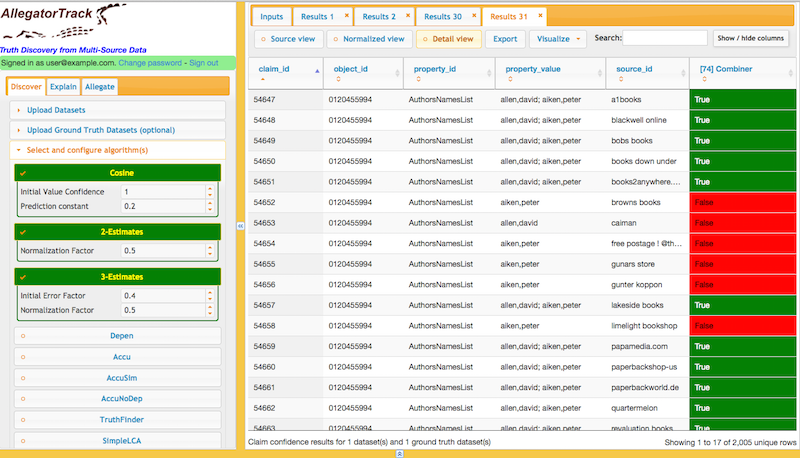
\includegraphics[scale=0.45]{snapshot} 
\caption{AllegatorTrack System}\label{allegatortrack}
\end{figure}

% Ongoing development
\section{Further Developments}
Currently, the API is still in improvements and many new other aspects of truth finding and endpoints are still under investigation, based on recent
proposed development in the field, discussions with early adopter developers, and users' feedbacks. For example, the scheme may support HTTPS in the 
future, the response body format may support other output formatting like XML.Most importantly, the API must be extended in the future in order to propose
broader class of truth finding algorithms, in particular the new ones.

% Questions or Feebacks
\section{Questions or Feebacks}
For any questions or feebacks about the API, please feel free to contact us %by email on \href{mailto:lberti@qf.org.qa}{dafna.qf.org.qa}
or visit the website of the DAFNA project for more details by following the link below:
\href{http://dafna.qcri.org}{\small{http://dafna.qcri.org}}.

\end{document}